\documentclass[tikz,border=5pt]{standalone}
\begin{document}
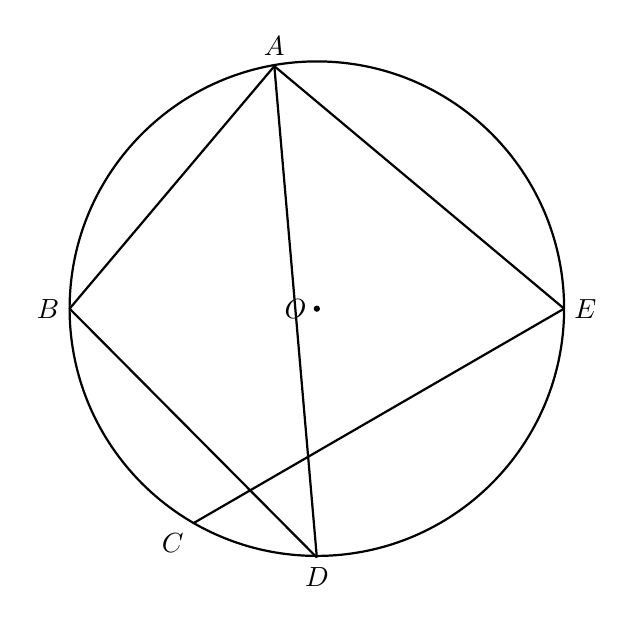
\begin{tikzpicture}[scale=1, line width=0.8pt]
  % 圆及圆心
  \coordinate (O) at (0,0);
  \draw (O) circle (3.14);
  \fill (O) circle (0.04);
  \node[left] at (O) {$O$};

  % 点坐标
  \coordinate (A) at (-0.54,3.08);
  \coordinate (B) at (-3.14,0);
  \coordinate (E) at (3.14,0);
  \coordinate (C) at (-1.56,-2.72);
  \coordinate (D) at (0,-3.16);

  % 原图线段
  \draw (A) -- (B);
  \draw (A) -- (E);
  \draw (B) -- (D);
  \draw (E) -- (C);

  % 编辑指令：实线段 AD
  \draw (A) -- (D);

  % 标签
  \node[above] at (A) {$A$};
  \node[left] at (B) {$B$};
  \node[right] at (E) {$E$};
  \node[below left] at (C) {$C$};
  \node[below] at (D) {$D$};
\end{tikzpicture}
\end{document}
